Il grafo è un insieme di coppie di vertici dove:
\begin{itemize}
    \item $<V,E>$ Dove $E = \{A  \subseteq\ V | |A| = 2\}$  questo significa che \textbf{E} è un insieme formato da coppie di \textbf{vertici V}
    \item Possiamo indicare un grafo come \textbf{G} quindi possiamo scrivere $G = <V,E>$
    \item Quindi \textbf{E} è la \textbf{relazione binaria} su \textbf{V} ossia $E \subseteq V$x$V$ quindi \textbf{E} è L'insieme degli archi che sono presenti nel grafo \textbf{G}
    \item In un grafo \textbf{orientato} le coppie in \textbf{E} sono ordinate , quindi $(X,Y) \neq (Y,X)$ in un grafo \textbf{non orientato} questa differenza non c'è. 
    \item Diciamo che $0 \leq |E| \leq |V|^2 - |V|$, facciamo \textbf{meno |V|} poiché non considerammo i \textbf{self loop}
    \item Due vertici che hanno una \textbf{relazione} si chiamano \textbf{adiacenti}, quindi se abbiamo la coppia $(X,Y)$ allora \textbf{X e Y} sono adiacenti.
    \item Un \textbf{Grafo è etichettato} se ogni vertice ha una \textbf{"Etichetta"} che lo distingue dai altri.
    \item un \textbf{ciclo è semplice} se e solo se il primo è l'ultimo vertici sono uguali
    \item un grafo senza cicli viene chiamato aciclico 
    \item Il \textbf{grado massimo di un grafo} è il \textbf{numero massimo di archi uscenti da un nodo}
\end{itemize}
\subsection{Cammini}
\begin{itemize}
    \item Un percorso chiamato anche \textbf{Path} è una sequenza di vertici $v_0,v_1,...,v_n$ purché esistono dei archi tra questi vertici , quindi $(v_i,v_{i+1}) \in E$ dove $1 \leq i \leq n-1$
    \item Un \textbf{Path} è \textbf{Semplice} se tutti i vertici del percorso sono distinti
    \item La lunghezza del percorso è data dal numero di archi attraversati
    \item Un \textbf{Path} è \textbf{ciclico} se il \textbf{primo e l'ultimo vertice si ripetono}, un percorso per essere ciclico deve avere almeno una lunghezza $\geq 3$
\end{itemize}

\subsection{Sotto Grafi}
\begin{itemize}
    \item Presi Due grafi \textbf{G} e \textbf{G'} dove $G = <V,E>$ e $G'=<V',E'>$
    \item Diciamo che \textbf{G'} è un \textbf{sotto grafo} se $V' \subseteq V$ e $ E' \subseteq E$
    \item Dciamo che \textbf{G'} è un \textbf{sotto grafo indotto} se $V' \subseteq V$ e $ E' = E \cap V'$x$V'$
\end{itemize}

\subsection{Componenti concesse e fortemente connesse}
\begin{itemize}
    \item Un \textbf{grafo} o un \textbf{sotto grafo} \textbf{non orientato} si dice \textbf{connesso} se ogni vertice del grafo o sotto grafo può raggiungere tutti i altri 
    \item formalmente Se \textbf{G non orientato} si dice \textbf{connesso} se: \newline \[\forall v,w \in V | (V,W) \in Reach(G)\] \newline dove \textbf{Reach} è L'insieme di \textbf{coppie di vertici che sono raggiungibili } Quindi se abbiamo (V,W) significa che V raggiunge W e che W raggiunge V(dipende anche dal grafo)

    \item Un \textbf{grafo} o un \textbf{sotto grafo} \textbf{orientato} si dice \textbf{fortemente connesso} se ogni vertice del grafo o sotto grafo può raggiungere tutti i altri 
    \item formalmente Se \textbf{G orientato} si dice \textbf{fortemente connesso} se: \newline \[\forall v,w \in V | (V,W) \in Reach(G)\] \newline dove \textbf{Reach} è L'insieme di \textbf{coppie di vertici che sono raggiungibili } Quindi se abbiamo (V,W) significa che V raggiunge W e che W raggiunge V(dipende anche dal grafo)
    \item  Invece quando parliamo di \textbf{componenti} stiamo parlando di un \textbf{sottoinsieme massimale}, quindi \textbf{Componenti concesse e fortemente connesse} in più hanno solo che \textbf{sono massimali} 
\end{itemize}

\subsection{Metodi di Rappresentazione}
Abbiamo due metodi di rappresentazione di un grafo:
\begin{itemize}
    \item  \textbf{Tramite matrice di adiacenza}
    \item  \textbf{Tramite liste di adiacenza} 
\end{itemize}
\subsubsection{Matrice di Adiacenza}
\begin{itemize}
    \item Matrice \textbf{|V| × |V|} di bit: 1 se esiste l’arco, 0 altrimenti.
\item Per rappresentare matrici pesate, ogni elemento contiene
un numero.
\item In ogni caso, richiede spazio $\theta(|V|^2)$
\item Tempo richiesto per aggiungere o rimuovere un altro vertice è di $\theta(|V|^2)$ poiché devo \textbf{creare} una nuova matrice e poi copiare gli elementi della \textbf{vecchia alla nuova}
\item La ricerca di adiacenti di \textbf{un vertice} è \textbf{lineare su |V|} quindi $O(|V|)$, invece per una \textbf{visita completa} è $\theta(|V|^2)$
\item cancellazione di un arco è constante.
\end{itemize}
\subsubsection{Liste di Adiacenza}
\begin{itemize}
    \item Vettore di \textbf{|V|} liste linkate (o altri contenitori più adeguati): la
    lista nella posizione \textbf{i-esima} contiene i vertici adiacenti a $V_i$
    (e in questo modo rappresenta gli archi).
    \item il vettore piu li liste linkate richiedono uno spazio di $\theta(|V| + E)$, ovviamente perchè l'array di \textbf{|V|} più le  listelinkate che tutte insieme possono essere massimo \textbf{|E|}.
    \item Per aggiungere o rimuovere un vertice il costo sarà di $\theta(|V|)$ poiché si dovrà allocare un vettore e non una matrice
    \item Per una ricerca dei \textbf{ADJ} di un vertice è $\theta(|E|)$
    \item Per una ricerca di tutto il grafo allora $\theta(|V| + |E|)$ quindi  io navigo tutto l'array \textbf{|V|} , dopo aver visionato tutto il grafo avrò visitato \textbf{|E|} archi. Diciamo che la somma di tutte liste di adiacenza di ogni vertice è \textbf{|E|}
    \item La cancellazione di un arco non è più constante può essere nel caso peggiore $O(|E|)$ nel caso migliore $\Omega(1)$
    
\end{itemize}

\subsubsection{Quando usere Una matrice o una lista di adiacenza}
Un grafo si dice:
\begin{itemize}
    \item Il grafo è \textbf{Denso:} se il numero di archi si avvicina a $\theta(|V|^2)$
    \item Il grafo è \textbf{Sparso:} se il numero di archi è più o meno $\theta(|V|)$
\end{itemize}
Ci conviene usare una \textbf{matrice} se il grafo è \textbf{denso} poiché occuperemo meno spazio , questo perché la lista di adiacenza per colpa dei puntatori per una grande quantità di archi  avrà tanti puntatori e cosi pesando di più. \newline
Al contrario se un\textbf{ grafo è sparso} allora ci conviene usare le \textbf{lista di adiacenza}, poiché sprecheremo meno spazio.
\subsection{Metodi Accessori}
\begin{itemize}
    \item In genere gli algoritmi prevedono di visitare i nodi adiacenti
    al nodo dato.
    \item Daremo supporto a questa necessità con due funzioni:
    \begin{itemize}
        \item \textbf{\textcolor{blue}{first(v)}} restituisce il primo vertice adiacente al
        nodo \textbf{v}, quindi il primo della lista
        \item \textbf{\textcolor{blue}{next(v,n)}} restituisce il vertice adiacente a \textbf{v}
        immediatamente dopo n nella lista dei nodi
        adiacenti;\textbf{ n = |V|} a fine lista.
    \end{itemize}
\end{itemize}
\begin{tcolorbox}[width=14cm, boxsep=10pt]
    \lstinputlisting{Capitoli/Grafi/Esempi/scorimento_lista.txt}
\end{tcolorbox}
\newpage
\subsection{Visite}
\begin{itemize}
    \item Come per gli alberi, anche per i grafi esistono delle visite
    \textbf{(traversals)} standard.
    \item  Ogni vertice viene visitato una sola volta.
\end{itemize}

\subsubsection{Problemi}
\begin{itemize}
    \item \textbf{Due problemi principali:}
    \begin{enumerate}
        \item grafo \textbf{non connesso}: non è possibile raggiungere tutti i
        vertici da quello scelto per partire;
        \item presenza di \textbf{cicli}, che possono portare, se non controllati, a
        loop infiniti.
    \end{enumerate}

    \item  Entrambi i problemi possono venir \textbf{risolti} con dei \textbf{marcatori}
    sui vertici (un bit per vertice):
    \begin{enumerate}
        \item  \textbf{cicli}: evito di visitare vertici già visitati;
        \item  grafo \textbf{non connesso}: alla fine controllo per vedere se ci
        sono vertici ancora non visitati (se ci sono, riparto con la
        visita da uno di questi)
    \end{enumerate}

\end{itemize}

\subsection{Implementazione Visita}
Quindi per vistare tutti i vertici dobbiamo \textbf{scorrere tutto il vettore} è se il \textbf{vertice} \textbf{non è stato vistato} allora vistare tutti i suoi \textbf{ADJ}\newline
\begin{tcolorbox}[width=14cm, boxsep=10pt]
    \lstinputlisting{Capitoli/Grafi/Esempi/BaseVisita.txt}
    \begin{itemize}
        \item Dove \textbf{doTraverse()} può implementare una visita in \textbf{ampiezza o
        in profondità.}
    \end{itemize}
\end{tcolorbox}

\subsection{Visita in ampiezza(BFS)}
\begin{itemize}
    \item \textbf{Breath-first search (BFS).}
    \item Prima di procedere visiti tutti i vertici collegati al vertice
    corrente.
    \item Struttura di supporto: \textbf{coda}.
    \lstinputlisting{Capitoli/Grafi/Esempi/BFScodice.txt}
\end{itemize}
\begin{center}
    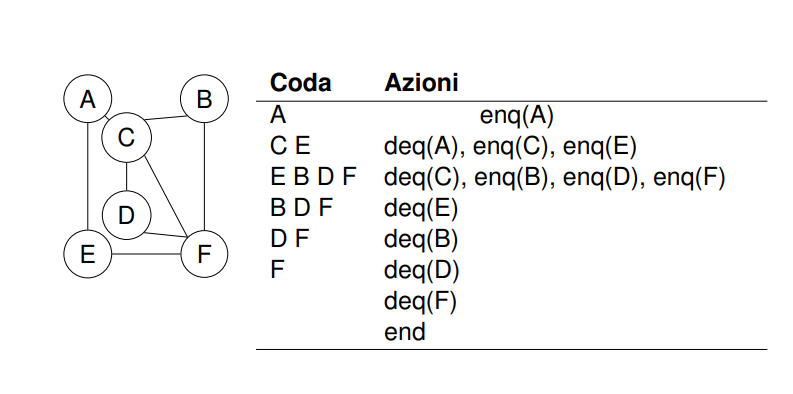
\includegraphics[scale = 0.6]{Capitoli/Grafi/Esempi/BFS.png}
\end{center}
\newpage
\subsection{Visita in profondità(DFS)}
Lo scopo della \textbf{DFS} è seguire il primo percorso del grafo finché non termina, nel momento in cui è terminato comincerà a risalire lo stack di esecuzione o di supporto finché non troverà una biforcazione. dopo aver trovato la biforcazione farà la stessa cosa che ha fatto al inizio , cioè percorrere tutto il percorso finché non termina. farà questo finché non visiterà tutto l'albero.
\begin{itemize}
    \item \textbf{Ricorsiva:} ogni volta che si visita un vertice \textbf{v} si visitano
    anche i suoi vicini non ancora visitati. però appena si trova un vicino non visitato entreremo in quel vicino e visteremo i suoi vicini, ripetiamo questo finché non troveremo nessun altro da esplorare
    \item \textbf{Iteratori}:
        \begin{itemize}
            \item si inseriscono in uno \textbf{stack} tutti gli archi che escono da \textbf{v};
            \item per \textbf{trovare il prossimo} vertice da visitare, si estrae e segue
            un arco dallo \textbf{stack}.
        \end{itemize}
        

    \item L’effetto è di seguire un ramo nel grafo fino alla sua
    conclusione prima di risalire le biforcazioni.
    \item Si costruisce così un \textbf{albero di ricerca in profondità.}
    \item \textbf{Vale sia per i grafi orientati che per quelli non orientati}
\end{itemize}
\newpage
\subsection{DFS Ricorsiva}
\lstinputlisting{Capitoli/Grafi/Esempi/DFSRicorsiva.txt}
\begin{center}
    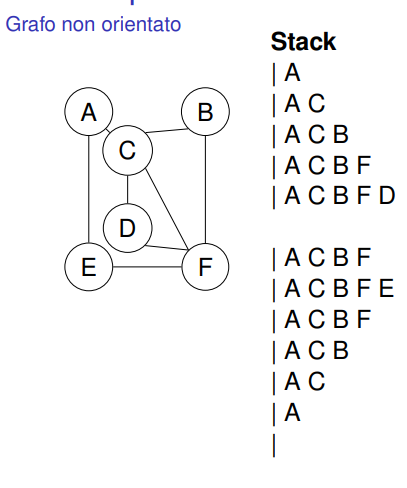
\includegraphics[scale = 0.6]{Capitoli/Grafi/Esempi/DFSNonOr.png}
\end{center}
\newpage
\subsection{DFS Iterativa}

\lstinputlisting{Capitoli/Grafi/Esempi/DFSIterativa.txt}
\begin{center}
    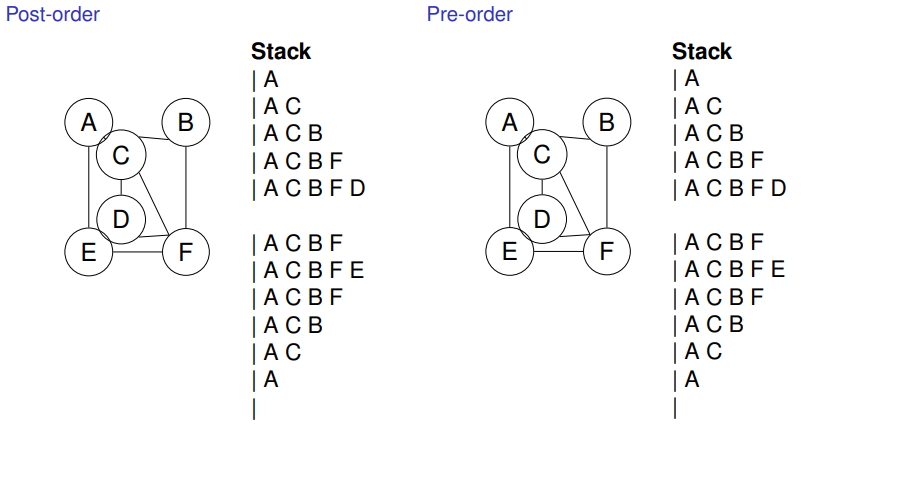
\includegraphics[scale = 0.6]{Capitoli/Grafi/Esempi/DFSIter.png}
\end{center}
Lo \textbf{stack non cambia} ma cambia solo l'ordine in cui viene effettuato il lavoro sul vertice

\newpage
\subsection{Foresta di visita}

\begin{center}
    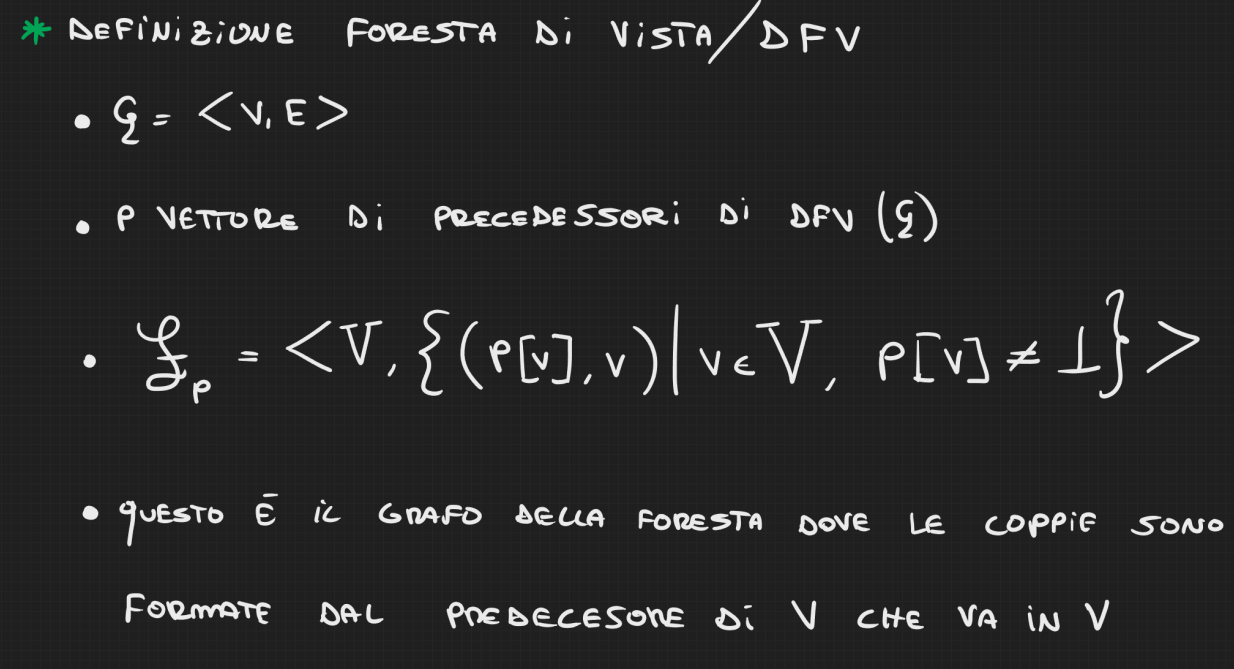
\includegraphics[scale = 0.5]{Capitoli/Grafi/Esempi/Foresta.png}
\end{center}
\subsubsection{Archi di Foresta}
\begin{center}
    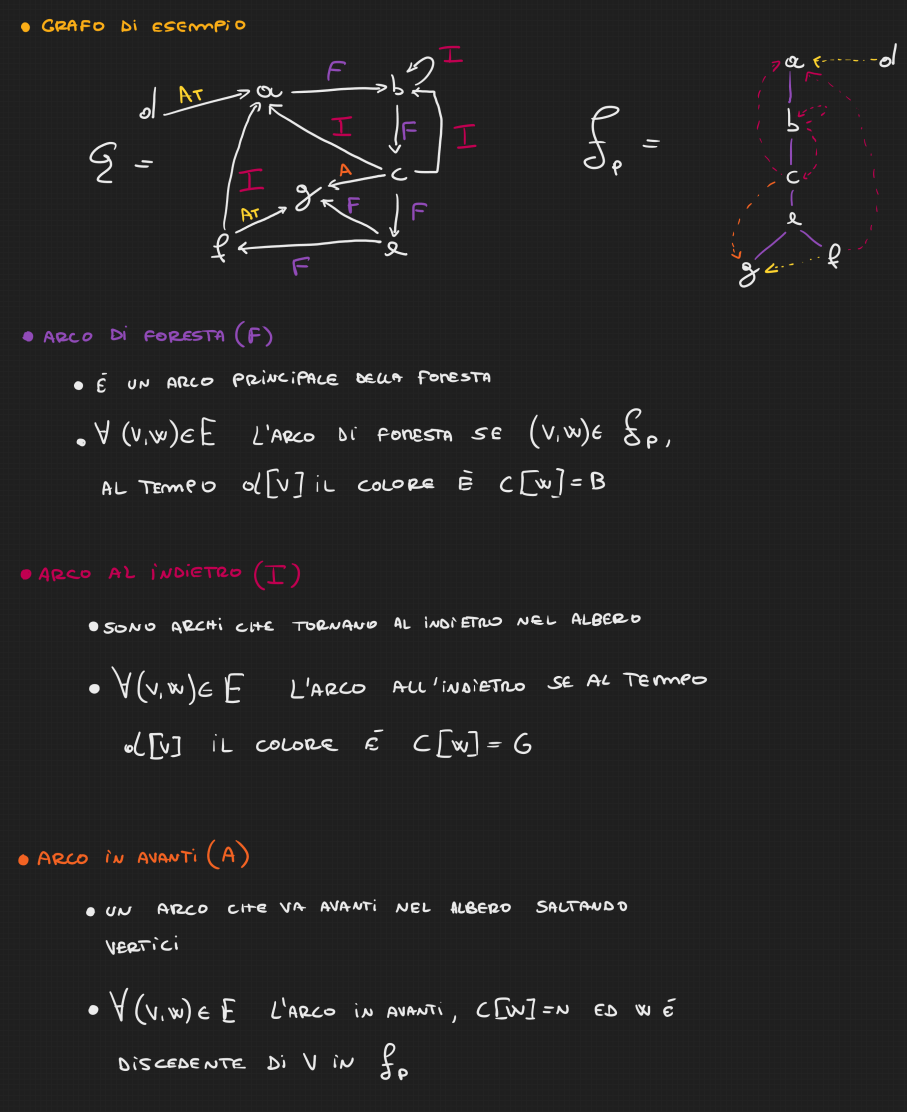
\includegraphics[scale = 0.6]{Capitoli/Grafi/Esempi/ArchiDiForesta.png}
\end{center}


